\section{Song aus Midi konvertieren}

Bisher haben wir manuell einen Song in einem Texteditor geschrieben. Für komplexere und längere Songs eignet sich das Konvertieren aus einer MIDI Datei. Ein Konverter übernimmt allerdings nur einen Teil unserer Arbeit. Die MIDI Datei muss vor dem Konvertiervorgang aufbereitet und das Ergebnis weiterhin im Texteditor bearbeitet werden.
\subsection{Vergleich der Konverter}
In diesem Kapitel werden drei Konverter vorgestellt, die alle Vor- und Nachteile mit sich bringen. Dabei handelt es sich um PetiteMM von gocha und loveemu, MIDI2MML von NeutronCat und mmltk von Nobody-86.
\subsubsection*{PetiteMM}
PetiteMM ist der mit Abstand älteste der drei Konverter mit einem simplen GUI.

\subsubsection*{Vorteile}
\begin{itemize}
	\item Java Programm lässt Benutzung auf Windows und MacOS zu
	\item Schneller Konvertiervorgang
	\item Konvertiert fast fehlerfrei
\end{itemize}

\subsubsection*{Nachteile}
\begin{itemize}
	\item Keine schöne MML Code Formatierung
\end{itemize}

\subsubsection*{MIDI2MML}
MIDI2MML ist ein neuerer Konverter aus Ende 2020.

\subsubsection*{Vorteile}
\begin{itemize}
	\item Benutzerfreundliches GUI
	\item Schneller Konvertiervorgang
	\item Schöne MML Code Formatierung
	\item Überlappende Noten werden über 8 Kanäle hinaus in separate Kanäle abgespeichert
	\item MIDI Events sind einsehbar
\end{itemize}

\subsubsection*{Nachteile}
\begin{itemize}
	\item C\# Programm, daher nur auf Windows zu benutzen
	\item Konverter interpretiert gewisse Notenwerte falsch
	\item Einige Notenwerte werden nicht intuitiv dargestellt.
\end{itemize}

\subsubsection*{mmltk}
mmltk ist ein weiterer neuerer Konverter aus Ende 2020, in Python geschrieben und als einziger Konsolenbasiert.

\subsubsection*{Vorteile}
\begin{itemize}
	\item Schöne MML Code Formatierung
	\item Überlappende Noten werden über 8 Kanäle hinaus in separate Kanäle abgespeichert
	\item Einziger Konverter der konstant fehlerfrei konvertiert
	\item Kann zusätzlich MML in eine MIDI Datei zurück konvertieren (experimentell)
\end{itemize}

\subsubsection*{Nachteile}
\begin{itemize}
	\item Programm momentan nur auf Windows zu benutzen
	\item Langsamer Konvertiervorgang
	\item Einmalige Installation aufwändiger als bei den anderen Konvertern
\end{itemize}

Da mmltk bei weitem das beste Ergebnis liefert, empfehle ich an dieser Stelle den einmaligen Mehraufwand der Installation.

\subsection{Installation und Benutzung von mmltk}
mmltk basiert auf Python, der erste Schritt ist also Python zu installieren.
Python kann hier heruntergeladen werden: \href{https://www.python.org/downloads/}{https://www.python.org/downloads/}

\bigskip

Als nächstes öffnen wir die Konsole und geben python -{}-version ein um zu testen, ob Python korrekt installiert wurde. Daraufhin sollte die Konsole mit der Versionsnummer von Python antworten.

\begin{figure}[htbp] \centering
	\includegraphics[width=.95\linewidth]{images/Python.png}
	\caption{Versionsnummer von Python aufrufen}
	\label{Python}
\end{figure}

mmltk benötigt 3 weitere Pakete die wir nun installieren und zwar mido, numpy und pandas.
Um die Pakete jeweils zu installieren, geben wir nacheinander

\bigskip

python -m pip install mido \\
python -m pip install numpy \\
python -m pip install pandas

\bigskip

ein. Ab jetzt können wir mmltk benutzen. Es kann unter \href{https://gitlab.com/Nobody-86/mmltk}{https://gitlab.com/Nobody-86/mmltk} heruntergeladen werden. \\
Nachdem wir die Datei an einem Ort unserer Wahl entpackt haben, öffnen wir wieder die Konsole.
Wir navigieren mit dem Befehl cd zu dem Verzeichnis, in dem mmltk.py liegt. Mit dem Befehl

\bigskip

python mmltk.py -i  \dq MIDINAME.mid\dq{} -o \dq MMLNAME.txt\dq{}

\bigskip

wird eine Midi in ein MML Dokument konvertiert, die im selben Verzeichnis liegt wie mmltk.py. \\
Alternativ kann auch der Pfad angegeben werden, falls die Midi nicht im selben Verzeichnis liegt wie mmltk.py. Tipp: Per Drag \& Drop wird automatisch der Dateipfad in die Konsole geschrieben.

\begin{figure}[htbp] \centering
	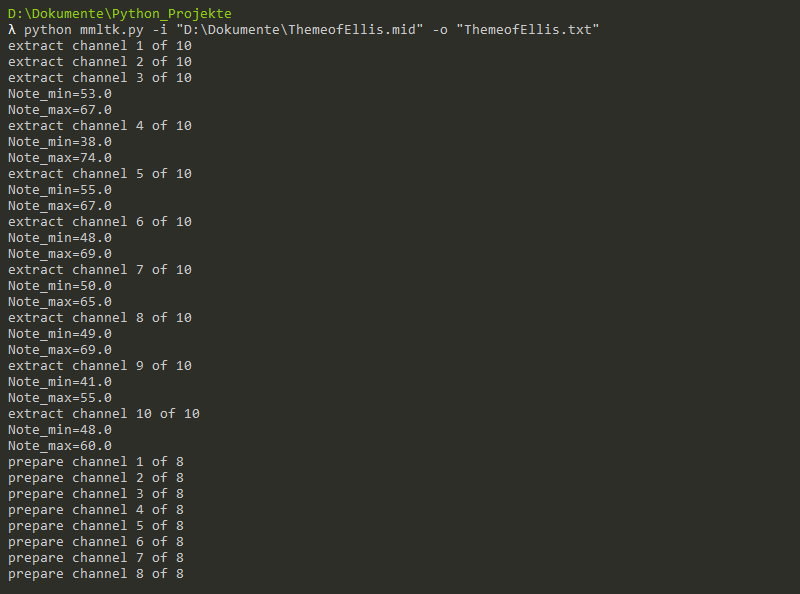
\includegraphics[width=.95\linewidth]{images/mmltk.png}
	\caption{MIDI mit mmltk in ein Textdokument mit MML konvertieren}
	\label{mmltk}
\end{figure}

\subsection{Midi aufbereiten und konvertieren}

Neben dem Konverter wird zusätzlich noch ein Programm benötigt, mit dem MIDIs (in einer Piano Roll) bearbeitet werden können. Beispiele dafür sind FL Studio, LMMS oder Anvil Studio. Die Trial Version von FL Studio reicht für unsere Zwecke vollkommen aus und beschränkt uns hinsichtlich des Arbeitens an Midi Dateien nicht. In diesem Tutorial benutze ich FL Studio und beschreibe den allgemeinen Umgang damit. \\
Wir öffnen eine beliebige MIDI Datei mit FL Studio, am einfachsten geht dies, indem die Datei per Drag \& Drop in das offene Programm gezogen wird. Wichtig hierbei ist, dass FL Studio nur MIDI Dateien mit der Endung .mid und nicht .midi öffnen kann. \\
Das folgende Fenster wird sich öffnen: 

\begin{figure}[htbp] \centering
	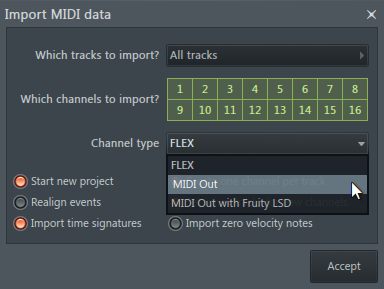
\includegraphics[width=.45\linewidth]{images/ImportMidi.png}
	\caption{MIDI mit FL Studio öffnen}
	\label{ImportMidi}
\end{figure}

Wir stellen den Channel type auf \textit{MIDI Out}. Falls zur MIDI Datei eine Soundbank in Form einer DLS (Downloadable Sound) Datei vorliegt, kann auch \textit{MIDI Out with Fruity LSD} ausgewählt werden. \textit{FLEX} sollte vermieden werden, besonders wenn man nur die Trial Version besitzt und keine FL Studio Projekte öffnen kann. FLEX Kanäle können notfalls auch im Nachhinein noch durch MIDI Out Kanäle ersetzt werden. \\
Als nächstes muss der MIDI Port geändert werden und zwar auf den gleichen, den auch die MIDI Out Kanäle verwenden (standardmäßig auf 0) Mit F10 öffnen sich die MIDI Settings, dort stellen wir den Port auf 0.

\bigskip

\begin{figure}[htbp] \centering
	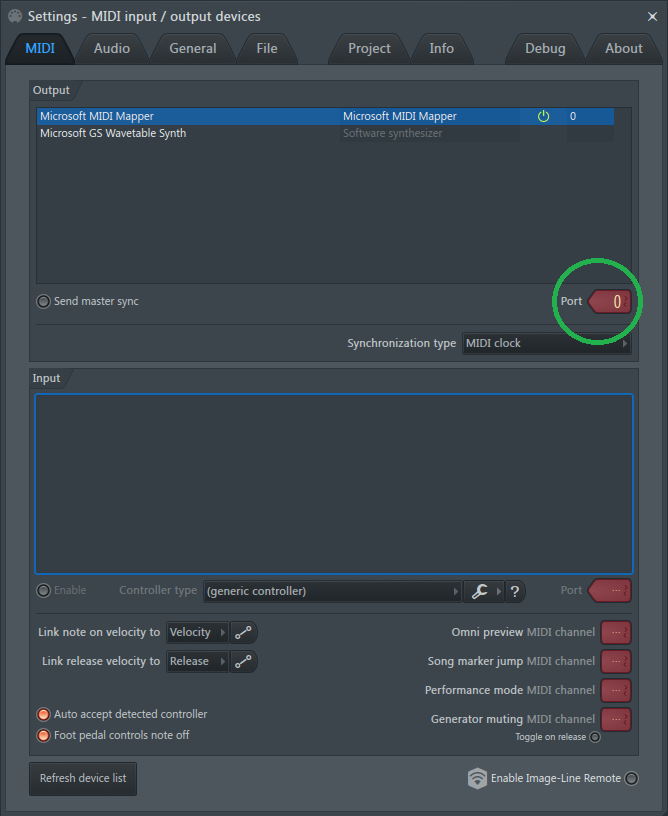
\includegraphics[width=.63\linewidth]{images/MIDIPort.png}
	\caption{MIDI Port wählen}
	\label{MIDIPort}
\end{figure}

Zusätzlich kann über den Reiter \textit{Project} die Timebase auf 48 PPQ eingestellt werden. Dadurch sind alle Noten und Pausen im richtigen Maß quantisiert, wodurch garantiert ist, dass die zeitliche Auflösung nie überschritten wird.

\bigskip

Ab jetzt sind alle Vorkehrungen getroffen und die MIDI Datei kann nach den bereits erwähnten Einschränkungen bearbeitet werden (pro Kanal nur eine Note gleichzeitig, maximal 8 Kanäle, Noten zwischen den Oktaven o1c bis o6a).
Zusätzlich sollte darauf geachtet werden, welche Noten in den Kanälen 7 und 8 liegen. Kanal 8 ist in SMW für den Sprung Soundeffekt reserviert, Kanal 7 für die restlichen Soundeffekte. Das hat zur Folge, dass vor allem lange Noten und Noten, die für eine markante Melodie zuständig sind, nicht in diesen beiden Kanälen untergebracht werden sollten. Jedes mal wenn ein Soundeffekt in SMW abgespielt wird, werden die Noten des entsprechenden Kanals stumm geschaltet.

\bigskip

Entspricht die MIDI Datei den Anforderungen, sollte das Projekt als .mid exportiert werden falls man nicht die Trial Version von FL Studio besitzt, weil man keine Projektdateien öffnen kann, MIDI Dateien aber schon (wie wir offensichtlich gesehen haben). \\
Hier sei noch einmal gesagt, dass man darauf achten soll, nicht FLEX zu benutzen, da es passieren kann, dass die exportierte MIDI Datei keine Noteninformationen enthält und alle Arbeiten verloren gehen.